%!TEX root=main.tex
\section{Effective Field Theories - Simplified Models - Concrete Models}
\label{sec:eftintro}

The Standard Model (SM) is the best currently available description of
fundamental interactions at the microscopic scale.\footnote{~Among the seminal papers are \citep{Weinberg:1967tq,Glashow:1961tr,Salammodel,Fritzsch:1973pi, Higgs:1964ia,Higgs:1964pj,Englert:1964et,Guralnik:1964eu, 'tHooft:1972fi}.}
It has been tested at experiments up to TeV energies, where the tests at the highest energies mainly come from the Large Hadron Collider (LHC). 
Within expected statistical fluctuations, the ensemble of these tests
supports the predictions of the SM to high precision.
Because the SM has a variety of internal and external deficiencies, it is expected that the SM is connected to a yet-unknown, more fundamental theory with new degrees of freedom at an energy $\Lambda$, somewhere between the TeV-scale tested at the LHC and the Planck scale, where gravity has to be accounted for. 
If $\Lambda$ is within the energy reach of the LHC, the BSM physics
will manifest itself in the form of new resonances and new or modified
interactions. If $\Lambda$ is above, but not too far above the TeV
scale, effects of BSM physics could still manifest themselves through
new effective interactions between SM fields. In the absence of any
clear deviations of experimental data from the SM predictions,
particle physics has developed several strategies to theoretically
approach BSM physics that will be discussed in this section:
expanding the SM into a SM-EFT in a bottom-up approach; a top-down
approach based on concrete BSM models; and a mixture of top-down and
bottom-up elements realized in simplified models.

Given the outstanding success of the SM, these approaches embed the SM, so that the Lagrangian 
for new physics can be schematically written as 
\begin{equation}
{\cal L}_{\rm new} = {\cal L}_{\rm SM} + {\cal L}_{\rm BSM}.
\label{eq:BSM}
\end{equation}
The different approaches to BSM physics differ in how ${\cal L}_{\rm BSM}$ is 
conceptualized.\footnote{Terms that include both SM and BSM fields are included in ${\cal L}_{\rm BSM}$.}
We will briefly summarize them in the following, with special emphasis on the SM-EFT.  


% =========
\subsection{BSM models}

During the past decades, BSM searches at the LHC and elsewhere
were mostly guided by models that postulate specific new concepts to solve open issues of the SM, e.g.\
new symmetries, new interactions, or new spatial dimensions at some energy scale $\Lambda $. 
Prominent examples of such models are supersymmetry~\citep{Wess:1974tw}, a new
symmetry between fermions and bosons, technicolor
models~\citep{Weinberg:1975gm,Susskind:1978ms}  which assume a new strong interaction, and
the Randall Sundrum model~\citep{Randall:1999ee} with an extra spatial dimension.  
These new concepts might be realized in a fundamental theory at (much) higher energies than the SM. However, in a top-down approach
observable deviations from the SM expectations at LHC energies, like new particles or 
modifications of cross sections, can be deduced in these models. 

Consider, for example, the case of supersymmetry (SUSY).
Supersymmetry is the largest possible extension of the Poincar\'{e}
group. This concept
leads to the idea of a symmetry between fermions and
bosons. All the SM particles have supersymmetric partners with spins
differing by $1/2$. 
TeV-scale SUSY models have typically about 100 new parameters and could address many outstanding issues of the SM by providing gauge coupling unification, describing the nature of dark matter, and solving the hierarchy problem.
However, as of yet, no signal of SUSY has been found.  


% =========
\subsection{Simplified Models}
\label{sec:SimpMod}

Due to the complexity of full BSM models, like SUSY, systematic simplifications have been developed in recent years that facilitate
searches for BSM physics. 
The main idea is not to use a whole,
concrete BSM model, but focus on one or a few of its new
features~\citep[see, e.g.,][]{alwall2009,alves2011}. To achieve this
formally, one may consider scenarios where almost all the new particles of
a BSM model have masses larger than the energies probed at the current
collider. Only a few selected new particles with TeV-scale masses are
then treated as relevant for experimental and phenomenological considerations.

A prominent example is the decay of a supersymmetric top quark
$\tilde{t}$. In a complete SUSY framework, it can decay into a large
number of final states.  In a simplified model, one restricts, for example, the
decays to $\tilde{t}\rightarrow t\chi^0$ (see e.g.~\cite{Aaboud:2017ayj}), while all other particles
are assumed to be too heavy to be produced in the decay.  
Here $\chi^0$ is the lightest neutral supersymmetric particle and considered a candidate for 
dark matter since it interacts at most very weakly with normal matter.  
Such a
simplification has repercussions on the interpretation of a
measurement.  Restricting SUSY to just one (or two) particles takes
these out of the context of a specific model and just provides an
experimental signature without any relation to other processes in the
model. Here, the simplified model is motivated in a top-down way from
the supersymmetric model. While such a signature may be interpreted as a signal for
$\tilde{t}$, it can equally well come from other objects in other
models with an equivalent decay, e.g. scalar third generation
leptoquarks that decay into $t+\bar{\nu}_t$~\citep{Aad:2015caa} or a generic Dark Matter particle with affinity to the
top quark. In this spirit, simplified models can also be constructed
in a bottom-up way: by building final states comprised of
combinations of new particles with different quantum numbers,
independent of any theory predicting these particles and their interactions.



% ===========
\subsection{SM-EFT}

Effective field theories (EFTs) are of central importance in particle
physics \citep[see, e.g.,][]{Georgi:1994qn}. 
In this subsection, we will give an overview of their historical use and development in particle physics and introduce a recent prominent case in the search for deviations from the SM.


\subsubsection{A historical blue-print: weak interactions}
\label{ssec:Fermi}

The Fermi theory of weak interactions~\citep{Fermi1934}, which aimed to describe the nuclear $\beta $-decay
as a pointlike interaction of four fermions (a proton, neutron, electron and a neutrino),
may serve as successful application of  a bottom-up approach to new physics using EFT procedures,
although, when Fermi developed his formalism in 1933, the concept of a
Quantum Field Theory and hence the concept of an effective QFT was not
yet established. Therefore for the sake of this discussion it is useful to translate Fermi's Ansatz
into the language of a modern QFT.
Here, we also replace neutrons and protons by quarks and include the 
helicity structure of the interaction. Then, the Fermi-interaction can
be written as
\begin{equation}\label{eq:Fermi}
{\cal L}_{\rm Fermi} = -\frac{G_F}{\sqrt2}\bar\nu\gamma^\mu(1-\gamma^5)e\,\bar q\gamma_\mu(1-\gamma^5)q'\,.
\end{equation}
The quark, electron and neutrino field operators are denoted by $q,\ q',\ e$ and $\nu$, respectively, and $\gamma^\mu, \gamma^5$ are the Dirac gamma matrices. 
The strength of the interaction is set by the Fermi constant $G_F = 1.15 \times 10^{-6}$~GeV$^{-2}$. 
In the decades following Fermi's approach to $\beta $-decay, the formalism  was successfully applied to the decay of the muon, and  to transitions between quarks. 
Fermi theory allowed one to include parity-violating couplings of weak interactions after its discovery in nuclear transitions, to understand special parameters to describe transitions between hadrons (CKM matrix), and serves to measure the mass of $\nu_e$. 
Thus, beyond describing just one process, the Fermi theory was a way to describe all weak interaction processes at low energy and the formalism of Fermi became the standard representation of low energy weak interactions. 
The Fermi theory has all features of an EFT. It provides an efficient
set of principles to organize weak interactions, allows one to compute
production rates and is manifestly incomplete. The latter is evident
as the Fermi coupling $G_F$ is dimensionful so that production rates
calculated within the Fermi theory will violate the probabilistic
interpretation of quantum theory (`unitarity violation') at
some energy $\Lambda \gg E_{\mathrm{\beta-decay}}$. For the Fermi
theory, this unitarity violation occurs at a centre-of-mass energy of
$E_{\rm unit.\, viol.}\approx \sqrt{1/G_F} \approx
300\,\mathrm{GeV}\gg E_{\mathrm{\beta-decay}}$. Thus, at energies near
$E_{\rm unit.\, viol.}$ new phenomena will occur and the Fermi theory
has to be replaced by a more fundamental theory. 

These phenomena are the existence of the $W$ and $Z$ bosons and the
electroweak interaction in the SM.
The Fermi theory is a low-energy limit of the electroweak theory of the SM, where interactions among 
fermions are mediated by the exchange of a virtual $W$ boson
with mass $m_W$ of about 80 GeV, and a 
coupling strength $g$ (see Fig.~\ref{fig:weak}, left). 
By including a $W$ propagator, the production rate is damped and unitarity violation is avoided.
\begin{figure}[htbp]
\begin{center}
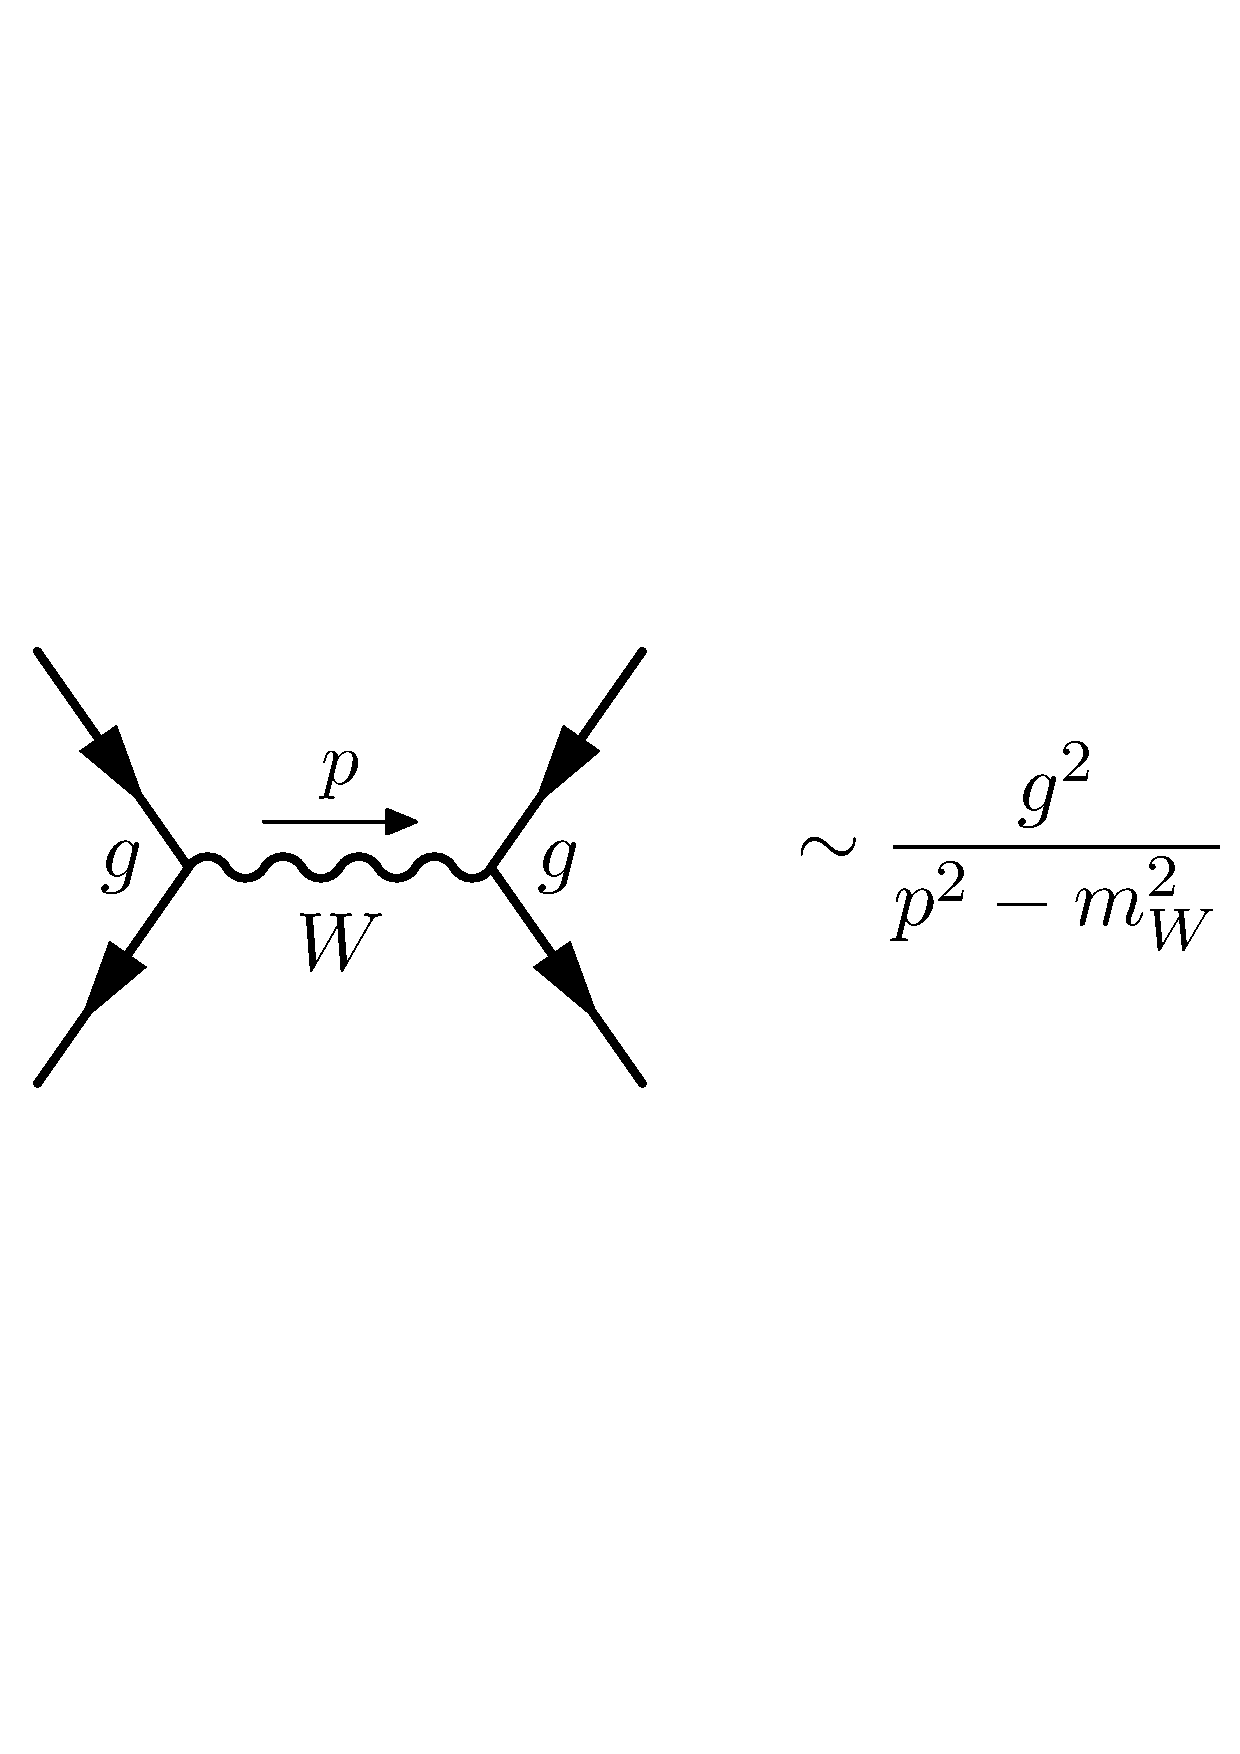
\includegraphics[width=0.4\textwidth]{weak_SM}\qquad\qquad
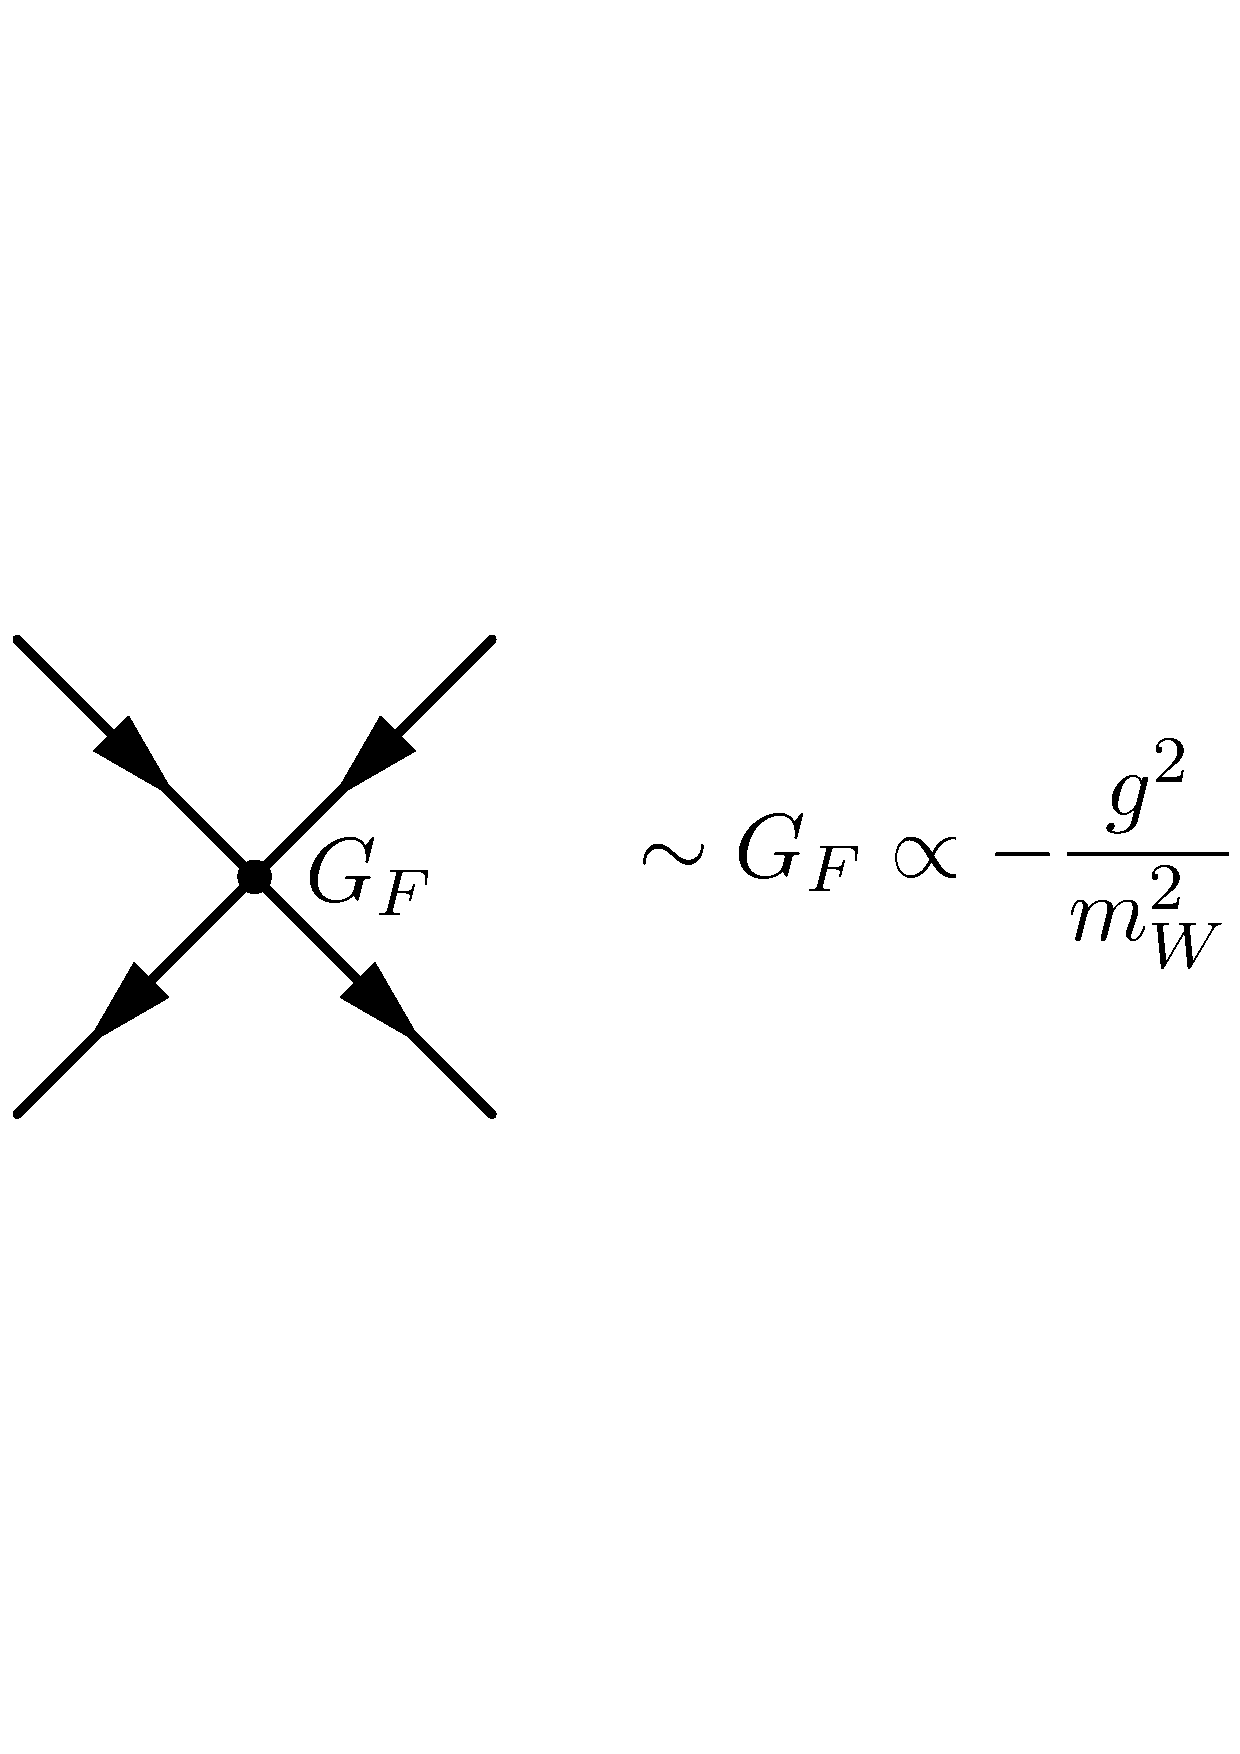
\includegraphics[width=0.4\textwidth]{weak_Fermi}
\caption{Weak interactions as described in the Standard Model (left) and in Fermi's four-fermion theory (right).}
\label{fig:weak}
\end{center}
\end{figure}
For momenta small compared to the mass of the $W$-boson, $p^2\ll m_W^2$, the $W$-propagator can be expanded in powers of $p^2/m_W^2$:
\begin{equation}
\frac{g^2}{p^2 - m_W^2} = -\frac{g^2}{m_W^2}\left(1 + \frac{p^2}{m_W^2}+{\cal O}\left(\frac{p^4}{m_W^4}\right)\right) \approx -\frac{g^2}{m_W^2} \equiv -\frac{G_F}{\sqrt2}\,.
\label{eq:wprop}
\end{equation}

Thus, the SM becomes equivalent to a pointlike effective four-fermion interaction with a strength set by the Fermi constant $G_F$ (Fig.~\ref{fig:weak}, right). 
This is an example of a \textit{top-down approach}, where the EFTs can be derived from a more fundamental theory formulated at higher energy scales.
From a modern perspective---i.e., assuming the availability of the formalism of QFT but not the SM---the Fermi theory could be regarded as an
early example for a \textit{bottom-up} EFT. 
On the other hand, the SM could not be unambiguously inferred from the Fermi theory, and neither
could the energy scale at which the EFT description breaks down, since $G_F$ depends 
on both the new scale and the unknown coupling $g$. 


% =========
\subsubsection{The Standard Model Effective Field Theory} \label{sec:smeftphysics}


In analogy to the Fermi theory, new effective interactions could be added
to the SM to describe a yet unknown theory of physics beyond the SM at
an energy scale $\Lambda$. In case of the Fermi theory, the new scale
was set by the $W$ boson mass, $\Lambda = m_W \approx 80$\,GeV. Since the structure and the
scale of physics beyond the
SM is not known, physicists adopt a
general bottom-up EFT to systematically evaluate potential BSM
effects at an energy scale $E_{\rm LHC}$  relevant for LHC physics. In the case of the
so-called 
Standard Model Effective Field Theory (SM-EFT)\footnote{See \cite{Buchmuller:1985jz,Grzadkowski:2010es} and the recent review
\cite{Brivio:2017vri}}, one assumes that the
new physics respects the SM gauge symmetries and that the scales are
well separated, $\Lambda\gg E_{\rm LHC}$. Note, however, that the
scale $E_{\rm LHC}$ depends on the physics process under
consideration, and thus the scale separation may not always be fulfilled in an LHC analysis. 

The SM-EFT describes a different phenomenology than the simplified
models or specific BSM models described above, where it is assumed that the masses of the new
particles and the experimental energy scale $E_{\rm LHC}$ are of the same
order of magnitude. In particular, this means that the SM-EFT does not
explicitly include new particles as dynamical degrees of freedom, but
assumes that any new particles would be too heavy to be directly produced in LHC experiments. 


The SM-EFT combines the SM fields to form all gauge invariant operators
${\cal O}_i^{(D)}$ with mass dimension $D$ and expands the SM
Lagrangian to
\begin{equation}
{\cal L}_{\rm SM-EFT} = {\cal L}_{\rm SM} + \sum_i c_i^{(6)} {\cal O}_i^{(6)} + \sum_j c_j^{(8)} {\cal O}_j^{(8)} + \ldots
\label{eq:smeft}
\end{equation}
The corresponding strength of the interaction is denoted by
$c_i^{(D)}$, where $c_i^{(D)} \ = \ (g_i^D/\Lambda^{D-4})$.\footnote{
  As the Lagrangian should have mass dimension four, such that the
  action $S = \int d^4x {\cal L}$ has mass dimension zero (in natural
  units $\hbar =c =1$), the coefficients $c_i^{(D)}$ must have mass
  dimension $4-D$.}  In the lowest relevant dimension D = 6, the
SM-EFT contains 2499 independent operators ${\cal O}_i^{(6)}$ as well
as 2499 $c_i^{(6)}$. It is important to note that there is a freedom
of choice of which set of independent operators 
is chosen. Each independent set is called a \emph{basis}. Depending on
the choice of basis, the SM-EFT predicts different sets of 
experimental observables to be theoretically connected through the same
operators~\citep[see, e.g.,][]{Falkowski:2015wza}. Consequences of
this freedom will be further discussed in
Section~\ref{sec:classification}. 

It should be noted
that the SM-EFT expansion, eq.~(\ref{eq:smeft}), is not an expansion in $\Lambda$
itself, but in $c_i=g_i/\Lambda$. 
In consequence, experimental constraints on deviations from the SM can
only be provided in terms of $g_i/\Lambda$.
As already discussed in the framework of the Fermi theory, one
does not immediately know the (bounds on the) scale of new physics, 
for which one would have to know $g_i$.
However, there are general constraints on the theoretical applicability of SM-EFT.
Since new resonances lead to significant contributions that cannot be captured by
the SM-EFT, the SM-EFT fails to describe physics distributions close to such a new resonance.
While in principle this makes the range of validity of the SM-EFT model dependent, 
it is generally assumed that $g \sim {\cal{O}}(1)$, such that the effects of the new 
resonance(s) with mass ${\cal{O}}(\Lambda)$ become visible already at
scales much smaller than $\Lambda$; thus one requires the SM-EFT to be valid at 
$\Lambda\gg E_{\rm LHC}$. 
For our further discussion we will assume such a strong separation of scales.
The intricacies of the range of validity of the SM-EFT are discussed,
for example, in~\cite{Contino:2016jqw}.




As mentioned above, this formalism is equivalent to what has been discussed for the Fermi theory. 
In fact some of the operators in Eq.~\ref{eq:smeft} are formally identical to the one of Eq.~\ref{eq:Fermi}. 
As in the Fermi theory the operators in the SM-EFT violate
unitarity, albeit at a scale of ${\cal O}(\gg TeV)$ (depending on the
parameter choices) instead of $\approx
300$\,GeV for the Fermi theory. Thus again, the SM-EFT is only an approximation and
involves two distinct mass scales, the one of the SM and a much larger scale of BSM physics.


% =========
\subsection{A Brief on the Physicists' Attitude}
\label{sec:physrepres}

The physicists' turn towards using the general SM-EFT formalism is borne out of the conceived dead end of expressing ideas for new physics in terms of concrete models.
This attitude is characterized, for example, by \cite[p.~1]{Contino:2013kra}:
``In absence of a direct observation of new states [i.e.{} particles], our ignorance of the EWSB sector can be parametrized 
in terms of an effective Lagrangian''.
It is beyond this paper to discuss in depth the epistemic and pragmatic goals of physicists leading to such a characterisation.
Suffice it to note, especially in view of the following discussions, that the bottom-up EFT approach is considered as being ignorant with respect to the nature of a `new state'.

What we consider important here is that a new state would have
definite properties to be scrutinized experimentally and theoretically, which is not the case for the general EFT approach.
If an experiment would find a new state, it would have definite properties that have to be represented in theory, e.g.\ by a field $\chi $.
Vice versa, if theory would propose a new state, its properties would largely be fixed and
would provide a clear target for experiments to search for.
In this case the field $\chi $ would be a representation of a new, but
not yet observed, particle.
In contrast, as will be detailed in Sect.~\ref{sec:classification}, the EFT approach
does not start from definite properties and thus neither provides
a clear target for experimentation, nor does it represent anything.  
In contrast to SM-EFT and global EFT approaches, concrete BSM models and simplified models
do assume fields or vertices representing entities and processes, and thus offer a well defined search strategy. 
It is such BSM theories that physicists ultimately strive for (also for other reasons).
This does not render EFTs useless, but the relation between these EFTs and BSM models becomes
apparent, for example in~\cite[p.~305]{deFlorian:2016spz}: the
``main motivation to use this framework is that the constraints on the EFT parameters can be 
later re-interpreted as constraints on masses and couplings of new particles in many BSM theories.''
Thus, while using EFT as a tool to parametrise constraints due to the (non)-observation of deviations
from the SM, most physicists want to reach beyond and arrive at a consistent and concrete BSM model.
